\section*{Sorted linked lists}

Hyrum's data structure involves sorted linked lists of integers
without duplicates.
% This is an invariant that should be maintained throughout the lab
% --- all linked lists must be sorted and \textbf{must not contain
% duplicates}.
Another thing that's different from the linked
lists that you've seen in lecture and homework is that there is no
``dummy node'' at the end of the list.  The end of the linked list is
reached when the \lstinline'next' pointer on a node is
\lstinline'NULL'. Here's an example of Hyrum's data structure:
\begin{center}
  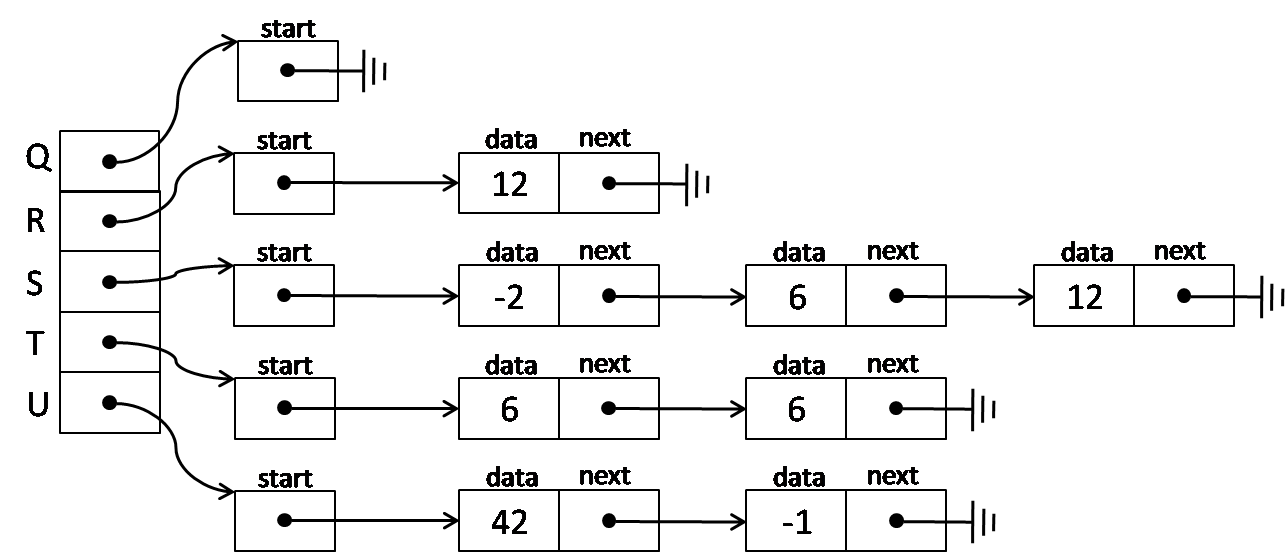
\includegraphics[width=0.93\textwidth]{\img/sortedlist.png}
\end{center}
In the illustration above, \lstinline'Q' is a sorted linked list
containing no numbers, \lstinline'R' contains just $12$, and
\lstinline'S' contains $-2$, $6$, and $12$. Neither \lstinline'T' nor
\lstinline'U' is a valid sorted linked list (for them,
\lstinline'is_sortedlist(T)' and \lstinline'is_sortedlist(U)' will
both return \lstinline'false').

The handout file \lstinline'listlib.c0'  contains declarations for the types
\lstinline'list' (identical to what we saw in class) and
\lstinline'sortedlist' (a struct pointing to a \lstinline'list' as in
the previous illustration).  It also contains the following
specification functions and helper functions, which may be useful
while testing.

% \textbf{You do not need to test the following six functions, they are guaranteed to be correct}.
\begin{lstlisting}
bool is_segment(list* start, list* end);
bool no_circularity(sortedlist* L);
bool is_sortedlist(sortedlist* L);
sortedlist* array_to_linkedlist(int[] A, int n)
  /*@requires 0 <= n && n <= \length(A) @*/ ;
int list_length(sortedlist* L)
  /*@requires L != NULL && no_circularity(L) @*/ ;
int[] linkedlist_to_array(sortedlist* L)
  /*@requires L != NULL && no_circularity(L) @*/
  /*@ensures list_length(L) == \length(\result) @*/ ;
bool arr_eq(int[] A, int[] B, int n)
  /*@requires 0 <= n && n <= \length(A) && n <= \length(B) @*/ ;
\end{lstlisting}
The function \lstinline'array_to_linkedlist' \textbf{naively}
constructs a linked list (not a sorted list) from an array.  Thus, if
we have an array \lstinline'A' equal to \lstinline'[-2, 6, 12]', then
\lstinline'array_to_linkedlist(A, 3)' would create the linked list
\lstinline'S' above.

The handout directory \lstinline'lab07' also contains Hyrum's five bad
implementations of \lstinline'sortedlist', named
\lstinline'sortedlist-bad1.c0', \lstinline'sortedlist-bad2.c0', etc.
Each defines the functions \lstinline'is_in', \lstinline'insert' and
\lstinline'delete'.

Your job for this lab will be to write exhaustive test cases for the
functions \lstinline'is_in', \lstinline'insert' and \lstinline'delete'
to catch the bugs in the broken implementations.  Write your tests in
the file \lstinline|sortedlist-test.c0| in the directory
\lstinline|lab07|.

You can compile and run your code with these commands (one for each bad file):
\begin{lstlisting}[language={[coin]C}, belowskip=0pt]
% make 1
% make 2
% make 3
% make 4
% make 5
\end{lstlisting}
\emph{(\lstinline'make' is a program that can help you compile
  code. You can Google it to learn more if you want.)}

Your code should indicate a problem for each of the bad
implementations. Figure out the exact line that causes that bug, and
then tell your TA both the line and the bug for credit.

\begin{part}\onePT[2.5ex]\TAGS{correctness, linked-list, safety, testing}
  Find the bugs in the first broken implementation (\lstinline'bad1').
\end{part}

\begin{part}\twoPT[2.5ex]\TAGS{correctness, linked-list, safety, testing}
  Additionally, find the bugs in the next two broken implementations
  (\lstinline'bad2' and \lstinline'bad3').
\end{part}

\begin{part}\threePT[2.5ex]\TAGS{correctness, linked-list, safety, testing}
  Finally, find the bugs in the remaining two broken implementations
  (\lstinline'bad4' and \lstinline'bad5').
\end{part}

\begin{solution}
\begin{itemize}
\item%
  This has a bogus implementation of \lstinline'is_in'.
\item%
  Line 23 should be \lstinline'L->start->data > n' as opposed to
  \lstinline'L=>start->data >= n'.
\item%
  On line 57 inside \lstinline'delete', the \lstinline'null' check is
  after the dereference. This is incorrect.
\item%
  The \lstinline'delete' implementation is bogus (line 58), and
  inserting to the end of the list causes an infinite loop.
\item%
  The recursive function is fine (I think), but the \lstinline'delete'
  wrapper itself sets \lstinline'cur' to the second element without
  checking the data field of the first, so it doesn't delete properly
  when it should be deleting the first element of the list.
\item[\bf Extra:]%
  There's also an extra bug in every implementation, so have students
  look for these subtle bugs if they finish the lab well before the
  period is over. This isn't needed for extra credit, but it's an
  interesting bug :)
\end{itemize}
\end{solution}

\enlargethispage{5ex}
\textbf{Some hints:}
\begin{itemize}
\itemsep=0pt
\vspace{-2ex}
\item%
  \textbf{To get the most out of this lab, don't spend a long time reading the
  bad implementations! Some of the bugs are quite subtle, and what we
  want to teach you is to write good tests.}
\item%
  Be thorough with your edge cases! Make
  sure the linked list behaves exactly as specified.
\item%
  Some implementations cause \lstinline'NULL' pointer dereferences.
  Others cause contract failures.  Others yet cause contract
  exploits. Make sure your tests can catch each of these types of bugs.
\item%
  Some bugs ``cancel'' each other out and make a list appear to work
  correctly and not fail any contracts.  The later versions of
  \lstinline'sortedlist' may have multiple errors!
\end{itemize}
